\begin{definition}[Rewriting framework \cite{endrullis2024generalized_arxiv_v2}]
  \label{def:rewriting_framework}
    A \textbf{DPO rewriting framework} $\mathfrak{F}$ is a mapping of DPO rewriting rules to collections of DPO diagrams. Specifically, for every rule \( \rho = (L \overset{l}{\leftarrow} K \overset{r}{\rightarrow} R) \), the collection $\mathfrak{F}(\rho)$ consists of DPO diagrams of the form shown below.
 \begin{center}
      \resizebox{0.4\textwidth}{!}{
      \begin{tikzpicture}
            \node (I) at (0,0) {$K$};
            \node (L)  at (-2,0) {$L$};
            \node (R)  at (2,0) {$R$};
            \node (G)  at (-2,-2) {$G$};
            \node (C)  at (0,-2) {$C$};
            \node (H)  at (2,-2) {$H$};
            \draw [->] (I) to  node [midway,below] {$l$} (L);
            \draw [->] (I) to  node [midway,below] {$r$} (R);
            \draw [->] (L) to node [midway,right] {} (G);
            \draw [->] (I) to  node [midway,right] 
            % {$u$}
            {} (C); 
            \draw [->] (R) to  node [midway,right] 
            {}
            (H);
            \draw [->] (C) to node [midway,above] {} (G);
            \draw [->] (C) to node [midway,above] 
            {} 
            (H);
        \end{tikzpicture}
        }
    \end{center}
    The \textbf{DPO rewriting relation $\Rightarrow_{\rho,\mathfrak{F}}$ induced by a DPO rewriting rule $\rho$ in $\mathfrak{F}$} is defined as follows: $G \Rightarrow_{\rho,\mathfrak{F}} H$ iff $G \Rightarrow_\rho^\delta H$ for some $\delta \in \mathfrak{F}(\rho)$. 
     The \textbf{DPO rewriting relation $\Rightarrow_{\mathcal{R},\mathfrak{F}}$ induced by a set $\mathcal{R}$ of DPO rewriting rules in $\mathfrak{F}$} is given by: $G \Rightarrow_{\mathcal{R},\mathfrak{F}} H$ iff $G \Rightarrow_{\rho,\mathfrak{F}} H$ for some $\rho \in \mathcal{R}$. When $\mathfrak{F}$ is clear from the context, we 
    suppress $\mathfrak{F}$ and 
    write $\Rightarrow_{\rho}$ and $\Rightarrow_{\mathcal{R}}$.
  \end{definition}
Let \(\mathfrak{F}\) denote the DPO rewriting framework that associates each rule \( \rho = (L \overset{l}{\leftarrow} K \overset{r}{\rightarrow} R) \) with the collection of all DPO diagrams of the form shown in~\autoref{def:rewriting_framework}.
Let \(\mathfrak{M}\) denote the DPO rewriting framework that associates each rule with the collection of all DPO diagrams of the following form with monic match $m$.
\begin{center}
           \resizebox{0.4\textwidth}{!}{
      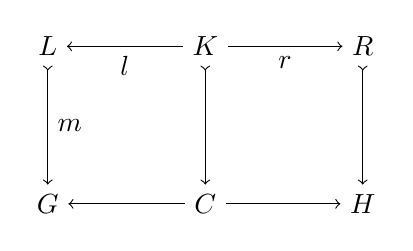
\begin{tikzpicture}
            \node (I) at (0,0) {$K$};
            \node (L)  at (-2,0) {$L$};
            \node (R)  at (2,0) {$R$};
            \node (G)  at (-2,-2) {$G$};
            \node (C)  at (0,-2) {$C$};
            \node (H)  at (2,-2) {$H$};
            \draw [->] (I) to  node [midway,below] {$l$} (L);
            \draw [->] (I) to  node [midway,below] {$r$} (R);
            \draw [>->] (L) to node [midway,right] {$m$} (G);
            \draw [>->] (I) to  node [midway,right] 
            % {$u$}
            {} (C);
            \draw [>->] (R) to  node [midway,right] 
            {}
            (H);
            \draw [->] (C) to node [midway,above] {} (G);
            \draw [->] (C) to node [midway,above] 
            {} 
            (H);
        \end{tikzpicture}
        }
    \end{center} 
     